\documentclass[12pt]{article}
\usepackage{tikz}
\usepackage{pgf-umlcd}
\begin{document}
\section*{Pr\'{a}ctica N}
Considere los siguientes archivos fuente
\begin{verbatim}
/**main.h*/
#ifndef MAIN_H
#include <iostream>
#include <vector>
#include <stdbool.h>
using namespace std;
#define NELEM(x)	((sizeof(x))/(sizeof((x)[0])))
typedef unsigned int uint;
extern unsigned int bucket[256];
/** suma de elementos
*/
unsigned int selem(unsigned int [NELEM(bucket)],int);
void fill_string_vec(string,vector<string>&);
void print_vector_string(vector<string>);
bool is_included(std::string,vector<string>);
bool is_space(char c);
#endif // MAIN_H
\end{verbatim}
\begin{verbatim}
/** funciones.cpp */
#include <iostream>
#include <vector>
#include "main.h"
using namespace std;

/** Suma los elementos del arreglo b y
 *  devuelve el resultado.
 */
uint selem(unsigned int b[256],int s)
{
  int i,suma=0;//,x,z;
  for(i=0; i<=(int)NELEM(bucket); i++)
  {
     suma=suma+b[i];
  }
  return suma;
}/*end selem()*/

/**Stub (inicialmente 2020.03.10)
 * Debe colocar en el vector string_vec las subsecuencias de
 * characters del string linea que no contienen characters ' '.
  pre:string_vec.size()=0
*/
void fill_string_vec(string linea,
                     vector<string>& string_vec)
{
  uint i,inic=-1,fin;
  std::string str_tmp;
  /**detect if string is fill of ' 's*/
  for(i=0;i<linea.size();i++)
  {
    if(linea[i]==' ')
        continue;
    inic=i;
    break;
  }
  if(inic<0)
    goto out;
  while(i<=linea.size()-1)
  {
    for(i=inic;i<linea.size();i++)
    {
      if(linea[i]==' ')
        continue;
      inic=i;
      break;
    }
    for(i=inic;i<linea.size();i++)
    {
      if((' '==linea[i])||('\0'==linea[i])||(i==(linea.size()-1))){
        fin=i;
        str_tmp=linea.substr(inic,fin-inic+1);
        
        //print_index_char_of_string(str_tmp);
        if(str_tmp.size()>=2){
          /**Quitar coma --si la hay--*/
          if(str_tmp[str_tmp.size()-2]==',')
            str_tmp=str_tmp.substr(0,str_tmp.size()-2);
          /**Quitar punto y coma --si lo hay--*/
          if(str_tmp[str_tmp.size()-2]==';')
            str_tmp=str_tmp.substr(0,str_tmp.size()-2);
          /**Quitar punto --si lo hay--*/          
          if(str_tmp[str_tmp.size()-2]=='.')
            str_tmp=str_tmp.substr(0,str_tmp.size()-2);
        }
        if(!is_included(str_tmp,string_vec))
          string_vec.push_back(str_tmp);
        inic=fin+1;
        break;
      }
    }/*end for()*/
  }/*end while()*/

out:
    return;
}/*end fill_string_vec()*/


void print_vector_string(vector<string> v)
{
    unsigned int i;
    for(i=0;i<v.size();i++)
    {
        cout<<v[i]<<"\n";
    }
}/*end print_vector_string()*/

bool is_included(std::string word,vector<string> word_list)
{
  for(uint i=0;i<word_list.size();i++)
  {
    if(word==word_list[i])
      return true;
  }
  return false;
}

bool is_space(char c)
{
  return (' '==c);
}

\end{verbatim}
y el archivo principal (archivo que contiene la funci\'{o}n main)
\begin{verbatim}
/**main0.cpp*/
#include <iostream>
#include <stdio.h>

#define NDEBUG
#include <assert.h>
#include "main.h"

using namespace std;
unsigned int bucket[256];

int main(int argc,char *argv[])
{
    uint i;
    char str[]="Pater noster, qui es in caelis, \
 santificetur nomen Tuum, adveniat Regnum Tuum, \
 fiat voluntas tua, sicut in caelo et in terra. \
 Panem nostrum cotidianum da nobis hodie, \
 et dimitte nobis debita nostra, \
 sicut et nos dimittimus debitoribus nostris; \
 et ne nos inducas in tentationem,\
 sed libera nos a malo";
    printf("%s\n",str);

    for(i=0;i<NELEM(str);i++)
    {
        bucket[(int)str[i]]++;
    }
    printf("suma=%d\n",selem(bucket,NELEM(bucket)));

    printf("%-4s %-6s\n","Char","Amount");
    for(i='A';i<='Z';i++)
    {
        if(bucket[i])
            printf("%c %5d\n",i,bucket[i]);
    }
    for(i='a';i<='z';i++)
    {
        if(bucket[i])
            printf("%c %5d\n",i,bucket[i]);
    }

    return 0;
}/*end main()*/

\end{verbatim}

\section*{Abstracci\'{o}n de operaciones}
N\'{o}tese que el c\'{o}digo en la funci\'{o}n {\tt main} del archivo {\tt main0.cpp} 
esencialmente utiliza la t\'{e}cnica buckets para contar cu\'{a}ntas letras may\'{u}sculas y 
min\'{u}sculas se utilizan en la cadena
\begin{verbatim}
    char str[]="Pater noster, qui es in caelis, \
 santificetur nomen Tuum, adveniat Regnum Tuum, \
 fiat voluntas tua, sicut in caelo et in terra. \
 Panem nostrum cotidianum da nobis hodie, \
 et dimitte nobis debita nostra, \
 sicut et nos dimittimus debitoribus nostris; \
 et ne nos inducas in tentationem,\
 sed libera nos a malo";
\end{verbatim}
Como ejercicio pr\'{a}ctico se le pide al lector reescribir la funci\'{o}n {\tt main} de ma\-ne\-ra 
que en lugar de contar cu\'{a}ntas letras may\'{u}sculas y min\'{u}sculas tiene la cadena {\tt str}, 
se haga la cuenta en la funci\'{o}n {\tt main} de cu\'{a}ntas veces aparece cada palabra en la misma 
cadena. Para responder al ejercicio pr\'{a}ctico el lector deber\'{a} utilizar la estructura que 
se describe a continuaci\'{o}n en la forma en que se le indicar\'{a} en este documento 
expl\'{i}citamente.

\subsection*{Primera modif\/icaci\'{o}n a la funci\'{o}n main}
Modif\/ique la funci\'{o}n main del archivo {\tt main0.cpp} para que quede como se indica a 
continuaci\'{o}n y guarde los cambios en el archivo {\tt main1.cpp}
\begin{verbatim}
/**main1.cpp*/
#include <iostream>
#include <stdio.h>

#define NDEBUG
#include <assert.h>
#include "main.h"

using namespace std;
unsigned int bucket[256];

int main(int argc,char *argv[])
{
    uint i;
    char str[]="Pater noster, qui es in caelis, \
 santificetur nomen Tuum, adveniat Regnum Tuum, \
 fiat voluntas tua, sicut in caelo et in terra. \
 Panem nostrum cotidianum da nobis hodie, \
 et dimitte nobis debita nostra, \
 sicut et nos dimittimus debitoribus nostris; \
 et ne nos inducas in tentationem,\
 sed libera nos a malo";
    printf("%s\n",str);

    for(i=0;i<NELEM(str);i++)
    {
        bucket[(int)str[i]]++;
    }
    printf("suma=%d\n",selem(bucket,NELEM(bucket)));

    printf("%-4s %-6s\n","Char","Amount");
    for(i='A';i<='Z';i++)
    {
        if(bucket[i])
            printf("%c %5d\n",i,bucket[i]);
    }
    for(i='a';i<='z';i++)
    {
        if(bucket[i])
            printf("%c %5d\n",i,bucket[i]);
    }
    
    vector<string> vs;         /*vector string*/
    string stringsa=string(str);
    fill_string_vec(stringsa,vs);
    printf("/******************************************/\n");
    print_vector_string(vs);

    return 0;
}/*end main()*/

\end{verbatim}
\subsection*{Una estructura string y uint}
En esta subsecci\'{o}n se describe una estructura que estar\'{a} formada por un {\tt string} 
y un {\tt unsigned int}. Se pide al lector utilizar el tipo de dato {\tt string} y el tipo 
de dato {\tt uint} def\/inido en el archivo {\tt main.h} como
\begin{verbatim}
typedef unsigned int uint;
\end{verbatim}
Agregue al archivo {\tt main.h} la declaraci\'{o}n de la estructura {\tt StringYuint} cuyo 
diagrama UML se incluye a continuaci\'{o}n.
\begin{center}
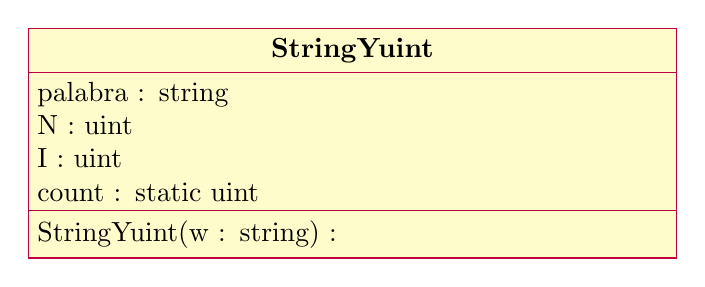
\begin{tikzpicture}
  \begin{class}[text width=8cm]{StringYuint}{0,0}
    \attribute{palabra : string}
    \attribute{N : uint}
    \attribute{I : uint}    
    \attribute{count : static uint}
    \operation{StringYuint(w : string) : }
    %\operation{entradaDatos( ) : void}
    %\operation{salidaDatos( ) : void}
    % virtual operations
    %\operation[0]{name(parameters list) : type of value returned}
    %\operation[0]{calcularArea() : void}
  \end{class}
\end{tikzpicture}
\end{center}
El lector deber\'{a} instanciar una estructura {\tt StringYuint} por cada palabra distinta 
que est\'{e} contenida en la cadena {\tt str}; el atributo de clase {\tt count} deber\'{a} 
inicializarse a cero en alcance de archivo. En el constructor de la estructura se 
incrementar\'{a} el valor del atributo de clase {\tt count} y se guardar\'{a} su valor en 
el atributo de objeto I. El atributo {\tt palabra} contendr\'{a} una de las palabras de la 
cadena {\tt str} y el atributo {\tt N} contendr\'{a} la cantidad de veces que aparece esa 
palabra en la cadena {\tt str}. N\'{o}tese que las distintas palabras contenidas en la cadena 
{\tt str} ya han sido colocadas en el vector de strings {\tt vs} del archivo {\tt main1.cpp}.
\subsection*{Instanciaci\'{o}n de las estructuras {\tt StringYuint}}
Una vez que el lector haya declarado la estructura {\tt StringYuint} en el archivo {\tt main.h} 
y agregado a ese mismo archivo de cabecera las l\'{i}neas
\begin{verbatim}
extern uint *BUCKET;
uint mapa(string word,StringYuint *syu_pt,uint size);
void contar_palabras(string line,StringYuint *syu_pt,vector<string> vs);
\end{verbatim}
se podr\'{a}n instanciar las estructuras correspondientes a las distintas palabras como se pide 
a continuaci\'{o}n en la funci\'{o}n {\tt main}: guarde los cambios en un archivo llamado 
{\tt main2.cpp}.
\begin{verbatim}
/**main2.cpp*/
//...
uint *BUCKET;

int main(int argc,char *argv[])
{
//...
    
    vector<string> vs;         /*vector string*/
    string stringsa=string(str);
    fill_string_vec(stringsa,vs);
    printf("/******************************************/\n");
    print_vector_string(vs);
    
    StringYuint *syu_Pt=new StringYuint[vs.size()];
    for(uint index=0;index<vs.size();index++)
    {
      syu_Pt[index]=StringYuint(vs[index]);
    }
    BUCKET=new uint[vs.size()+1];
    contar_palabras(stringsa,syu_Pt,vs);

    printf("/******************************************/\n");
    for(uint index=0;index<vs.size();index++)
    {
      printf("%-15s %3d\n",
             &(syu_Pt[index].palabra[0]),
             BUCKET[syu_Pt[index].I]);
    }    
    
    return 0;
}/*end main()*/

void contar_palabras(string line,
                     StringYuint *syu_pt,
                     vector<string> string_vec)
{

}
\end{verbatim} 
\end{document}